\section{Clasificador}

\note{Una vez que tenemos una idea general de lo que se quiere hacer y que tenemos un conjunto de datos para trabajar, procederíamos a mostrar nuestra implementación del clasificador. Pero antes es necesario estar en contexto sobre las técnicas utilizadas en este trabajo, que son del área \textbf{Aprendizaje Automático}.}

\begin{frame}
    \frametitle{Aprendizaje Automático}

    \begin{itemize}
        \item Objetivo: hacer \emph{aprender} a una computadora.
        \item Aprendizaje \emph{supervisado}.
        \item En la \emph{clasificación} se intenta aprender la categoría de una entidad.
        \item Etapas: \emph{entrenamiento} y \emph{evaluación}.
    \end{itemize}
\end{frame}

\note{Aprendizaje Automático es un área que tiene como objetivo hacer \textbf{aprender} a una computadora.

A su vez nosotros nos vamos a concentrar en lo que es el aprendizaje \textbf{supervisado}, es decir, aprender en base a ejemplos claramente etiquetados. En nuestro caso se aprenderá en base a tweets etiquetados como Humor o como No humor.

La tarea particular que queremos realizar se llama \textbf{clasificación}, y esto es que queremos asignarle una etiqueta (Humor o No humor) a una instancia, a un tweet.}

\subsection{Clasificadores}
\begin{frame}
    \frametitle{Clasificadores}

    \begin{itemize}
        \item Un clasificador decide en base a \emph{características} y a ciertas suposiciones.
    \end{itemize}
\end{frame}

\note{En cuanto a los clasificadores, ellos deciden en base a \textbf{características}, a valores, y además hacen suposiciones para generalizar cómo se comporta lo que se quiere buscar, en este caso el humor.

A continuación vamos a mostrar 4 técnicas que usamos en este trabajo, que hacen suposiciones distintas.}

\begin{frame}
    \frametitle{Support Vector Machine (SVM)}

    \begin{center}
        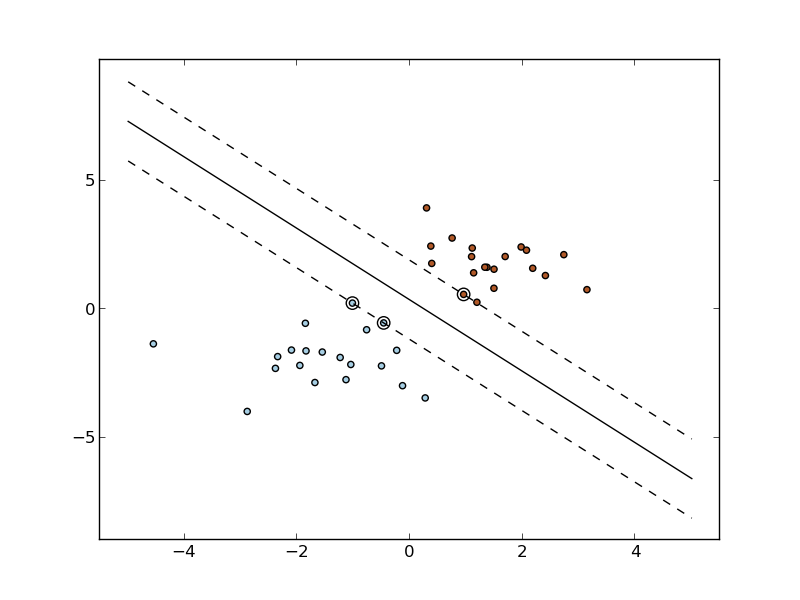
\includegraphics{svm.png}
    \end{center}
\end{frame}

\note{La primera técnica que mostramos es Suport Vector Machine o SVM.\@ SVM se basa en primero pasar las instancias a un espacio vectorial, en donde cada componente de cada tweet tiene el valor de una característica. Por ejemplo un tweet puede tener 1 en Ambigüedad y 3,5 en Jerga sexual. SVM intenta buscar la curva que mejor separe los ejemplos de las distintas clases.

Se muestra un ejemplo acá. En este caso el espacio vectorial es un plano y la curva elegida es una recta. Los ejemplos en este caso quedaron completamente separados, y es lo que supone SVM, pero no siempre ocurre esto.}

\note{Una vez que estamos en contexto con el área, procedemos a hablar de la implementación del clasificador.}

\subsection{Metodología}
\begin{frame}
    \frametitle{Metodología}

    \begin{itemize}
        \item Se utilizan SVM, kNN, DT, GNB y MNB.\@
        \item Se divide en 80\% entrenamiento y 20\% evaluación.
        \item Se usa validación cruzada sobre el conjunto de entrenamiento para resultados intermedios durante el desarollo y el conjunto de evaluación para el resultado final.
    \end{itemize}
\end{frame}

\note{Primero hablamos de la metodología que usamos. Se utilizan las técnicas, SVM, Vecinos más cercanos, Árboles de decisión y dos tipos de clasificadores Naïve Bayes: uno que supone que las probabilidades siguen una distribución gaussiana y otro que supone que siguen una distribución multinomial.

Dividimos el corpus en 80\% entrenamiento y 20\% evaluación. El corpus de evaluación lo dejamos para el final de manera de intentar no sesgarse demasiado a los resultados y que las métricas no sean mentirosas. Mientras se desarrollan las características y el clasificador se utiliza una técnica llamada validación cruzada para evaluar al clasificador. Cuando se quieren estudiar casos puntuales de error, como por ejemplo tweets falsos positivos, se ha partido nuevamente al conjunto de entrenamiento en entrenamiento y evaluación.}

\subsection{Línea base}
\begin{frame}
    \frametitle{Línea base}

    \begin{enumerate}
        \item BoW + MNB

        \item Clasificador que predice según lo que dice la mayoría (Negativo)
    \end{enumerate}

    \begin{center}
        \scriptsize
        \begin{tabular}{ c | r | r | r | r | r | r | r }
            & \multicolumn{1}{c |}{Precisión} & \multicolumn{1}{c |}{Recall} & \multicolumn{1}{c |}{$F_1$} & \multicolumn{1}{c |}{Prec. neg.} & \multicolumn{1}{c |}{Rec. neg.} & \multicolumn{1}{c |}{$F_1$ neg.} & \multicolumn{1}{c}{Acierto} \\
            \hline
            LB1 & \textbf{65,2} & \textbf{82,7} & \textbf{72,9} & \textbf{96,3} & 91,2 & \textbf{93,7} & \textbf{89,7} \\
            \hline
            LB2 & N/A & 0,0 & N/A & 82,5 & \textbf{100,0} & 90,4 & 82,5 \\
        \end{tabular}
    \end{center}
\end{frame}

\note{Decidimos establecer una línea base para comparar contra las técnicas utilizadas.

El primero de ellos es un modelo llamado Bag of Words, o bolsa de palabras. La idea es transformar cada tweet en un vector de conteos de las palabras que aparecen. Es decir, las características son cada una de las palabras que aparecen en los tweets. Un tweet por ejemplo puede tener la palabra ``mesa'' 2 veces, la palabra ``arte'' una vez y la palabra ``plato'' ninguna vez. Se combina esto con un clasificador Naïve Bayes multinomial.

El segundo es un clasificador mucho más simple. Se limita a predecir en base a la categoría que fue más frecuente en la etapa de entrenamiento. Dice lo que dice la mayoría, en otras palabras. En este caso dice que todo es negativo, No humor, porque observó al rededor de 83\% de negativos al entrenar.}

\note{Acá se muestran los números que se obtuvieron, en donde tenemos la Precisión [señalar], Recall, F1, lo mismo para los negativos y finalmente el acierto. Se puede observar que la primera línea base supera ampliamente a la segunda.}

\subsection{Características}

\begin{frame}
    \frametitle{Características}

    Qué se busca:

    \begin{itemize}
        \item Contradicción y negatividad
        \item Formato
        \item Informalidad
        \item Orientación en personas
        \item Temas recurrentes en chistes
    \end{itemize}
\end{frame}

\note{Básicamente buscamos las siguientes cosas: contradicción y negatividad en los tweets, determinado tipo de formato sintáctico, informalidad, que estén centrados en personas y temas recurrentes en chistes.}

\subsection{Características}
\begin{frame}[allowframebreaks]
    \frametitle{Características}

    \begin{center}
        \scriptsize
        \begin{tabular}{ c }
            Diálogo \\
            Distancia temática: Otros... \\
            Distancia temática: Atlantes \\
            Distancia temática: Chistes cortos \\
            Preguntas-respuestas \\
            Distancia temática: Adivinanzas \\
            Distancia temática: Animales \\
            Palabras clave \\
            Exclamación \\
            Hashtags \\
            Links \\
            Primera persona \\
            Segunda persona \\
            OOV Freeling \\
            Palabras mayúsculas \\
            Jerga sexual \\
            Negación \\
            OOV Wiktionary \\
            OOV Freeling Wiktionary \\
            Presencia de animales \\
            OOV Freeling Google \\
            Antónimos \\
            Palabras no españolas \\
        \end{tabular}
    \end{center}
\end{frame}

\subsection{Resultados obtenidos}
\begin{frame}
    \frametitle{Resultados obtenidos}

    \begin{center}
        \scriptsize
        \begin{tabular}{ c | r | r | r | r | r | r | r }
            & \multicolumn{1}{c |}{Precisión} & \multicolumn{1}{c |}{Recall} & \multicolumn{1}{c |}{$F_1$} & \multicolumn{1}{c |}{Prec. neg.} & \multicolumn{1}{c |}{Rec. neg.} & \multicolumn{1}{c |}{$F_1$ neg.} & \multicolumn{1}{c}{Acierto} \\
            \hline
            LB1 & \textbf{61,7} & \textbf{84,6} & \textbf{71,4} & \textbf{96,6} & 89,2 & 71,4 & \textbf{88,5} \\
            \hline
            LB2 & N/A & 0,0 & N/A & 83,0 & \textbf{100,0} & \textbf{90,7} & 83,0 \\
            \hline
            \hline
            SVM & 83,6 & 68,9 & \textbf{75,5} & 93,8 & 97,2 & \textbf{95,5} & \textbf{92,5} \\
            \hline
            DT & 66,5 & 67,5 & 67,0 & 93,3 & 93,0 & 93,2 & 88,9 \\
            \hline
            GNB & 57,5 & \textbf{78,2} & 66,3 & \textbf{95,2} & 88,2 & 91,5 & 86,5 \\
            \hline
            MNB & \textbf{84,8} & 60,0 & 70,3 & 92,3 & \textbf{97,8} & 95,0 & 91,4 \\
            \hline
            KNN & 81,3 & 66,3 & 73,0 & 93,4 & 96,9 & 95,1 & 91,7 \\
        \end{tabular}

        \begin{center}
            Mejor técnica: \textbf{SVM}
        \end{center}

        \begin{tabular}{ c | r | r }
            \textbf{son/clasif.} & Positivos & Negativos \\
            \hline
            Positivos & 842 & 381 \\
            \hline
            Negativos & 165 & 5805 \\
        \end{tabular}
    \end{center}
\end{frame}
